\documentclass{slides}

\lstset{language=C++}
\usepackage{array}
\usepackage{xspace}

\begin{document}
\newcommand{\ie}{\textit{i.\thinspace e.}\xspace}
\newcommand{\eg}{\textit{e.\thinspace g.}\xspace}

\graphicspath{{figures/}}

\title[Programming in C++: Outline]{\Large Programming in C++: Outline}

\author[A. Arnold and O. Lenz]{Axel Arnold \and Olaf Lenz} 
\institute{Institut für Computerphysik\\Universit\"at Stuttgart}
\date{March 17-21, 2014}

\setbeamertemplate{footline}{}
\begin{frame}
  \titlepage
\end {frame}
\setbeamertemplate{footline}[icp]

\begin{frame}
  \frametitle{General Information}
  \begin{itemize}
  \item ``Fachübergreifende Schlüsselqualifikation, Kompetenzbereich 1''
  \item 3 LP
  \item Requirement: Basic knowledge of programming\\ (C, FORTRAN \emph{or} Python)
  \item Lectures in the morning (9:15 - 12:30)
  \item Exercises in the afternoon (14:00 - 17:00)
    \begin{itemize}
    \item Mon: small exercises on Monday
    \item Tue-Fri: Team project: Edward
    \item Possibly a contest on Friday
    \end{itemize}
  \end{itemize}
\end{frame}

\begin{frame}
  \frametitle{Contents}
  \begin{itemize}
  \item Day 1
    \begin{itemize}
    \item Using C++
    \item Object-Oriented Design
    \item Compilation and Libraries (Tutorial)
    \end{itemize}
  \item Day 2
    \begin{itemize}
    \item A Tour of the Standard Library
    \item OOP in C++
    \item Test Driven Development in a Nutshell (Tutorial)
    \end{itemize}
  \item Day 3
    \begin{itemize}
    \item Getting Closer to the Metal: Pointers and Stuff
    \item OOP: Overloading, Inheritance and Polymorphism 
    \end{itemize}
    \item Day 4
      \begin{itemize}
      \item Exceptions and namespaces
      \item OOP in C++ 2
      \end{itemize}
    \item Day 5
      \begin{itemize}
      \item Templates
      \end{itemize}
  \end{itemize}
\end{frame}

\begin{frame}
  \frametitle{Recommended Literature}
  \begin{itemize}
  \item Best online ressource: \url{http://www.cplusplus.com}
  \item \textit{Thinking in C++: Introduction to Standard C++} by
    Bruce Eckel (Prentice Hall; 2nd edition; 2000)
    \begin{itemize}
    \item Free online book
    \item Good to learn about the ideas
    \item Meanwhile somewhat outdated
    \item ``TICPP''
    \item \dots what this course is based on
    \end{itemize}
  \item \textit{Thinking in C++: Practical Programming} by Bruce Eckel
    and Chuck Allison (Prentice Hall; 1st edition, 2003)
  \item \textit{The C++ Programming Language} by Bjarne Stroustrup
    (Addison-Wesley Professional; 4 edition, 2013)
    \begin{itemize}
    \item The reference for all things C++
    \item Includes new \textit{C++11} standard
    \item Not very good to \emph{learn} the language
    \end{itemize}
  \end{itemize}
\end{frame}

\begin{frame}
  \frametitle{History of C}
  \begin{columns}[c,onlytextwidth]
    \column{0.7\textwidth}
    \begin{tabular}{r<{:}p{0.8\textwidth}}
      1969 -- 73 & Developed by D. M. Ritchie (based on ``B'')\\
      1978 & ``\emph{The C Programming Language}'' by Kernighan und Ritchie (``K\&R'')\\
      1989 & Standard ANSI C89 = ISO C90\\
      1999 & Standard ISO C99\\
      2011 & Standard ISO C11
    \end{tabular}

  \begin{itemize}
  \item ``Procedural'' language
  \item Nowadays used mainly for system and embedded programming, \eg
    to implement
    \begin{itemize}
    \item Operating systems (\eg Unix, Windows)
    \item Other programming languages (\eg Python)
    \item \dots and in physics (only the young ones, the old ones use FORTRAN)
    \end{itemize}
  \end{itemize}

    \column{0.25\textwidth}
    \centering
    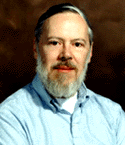
\includegraphics[height=0.25\textheight]{ritchie}\\
    {\tiny D. M. Ritchie, 1941 -- 2011}
    \vspace{\baselineskip}

    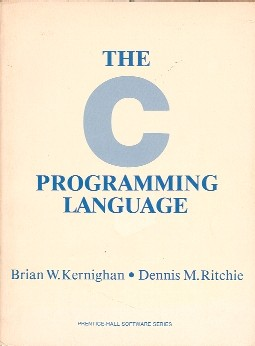
\includegraphics[height=0.4\textheight]{kr-c}\\
  \end{columns}
\end{frame}

\begin{frame}
  \frametitle{History of Object-Oriented Programming}
  \begin{columns}[c,onlytextwidth]
    \column{0.70\textwidth}
    \begin{tabular}{r<{:}p{0.9\textwidth}}
      1967 & \textit{Simula 67}: first object-oriented (OO) language
      by O. Dahl and K. Nygaard\\
      1971 & \textit{Smalltalk}: pure object-oriented language by
      A. Kay\\
    \end{tabular}
    \begin{itemize}
    \item Object-oriented programming is a \emph{programming paradigm},
      \ie a way to think about and implement programs
    \item OOP was a part of the solution to tackle the ``software
      crisis'' of the 1970s
    \item Most modern languages are OO (\eg Java, C\#, Python, \dots)
    \end{itemize}

    \column{0.25\textwidth}
    \centering
    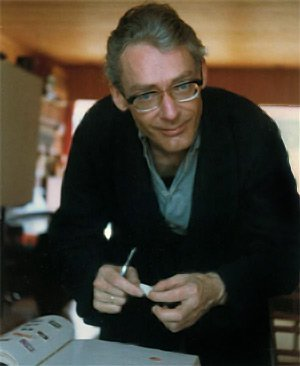
\includegraphics[height=0.25\textheight]{dahl}\\
    {\tiny O. Dahl, 1931 -- 2002}
    \vspace{\baselineskip}

    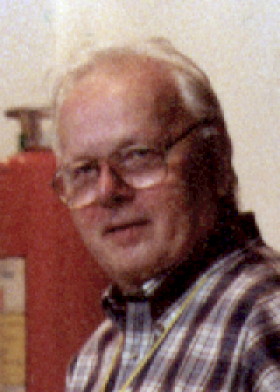
\includegraphics[height=0.25\textheight]{nygaard}\\
    {\tiny K. Nygaard, 1926 -- 2002}
  \end{columns}
\end{frame}

\begin{frame}
  \frametitle{History of C++}
  \begin{columns}[c,onlytextwidth]
    \column{0.6\textwidth}
    \begin{tabular}{r<{:}p{0.9\textwidth}}
      1979 & B. Stroustrup develops ``C with classes'' based on Simula 67\\
      1983 & Language is renamed to \textbf{C++}\\
      1985 & ``\emph{The C++ Programming Language}'' by Stroustrup\\
      1998 & Standard ISO C++98\\
      2011 & Standard ISO C++11
    \end{tabular}
    
    \column{0.25\textwidth}
    \centering
    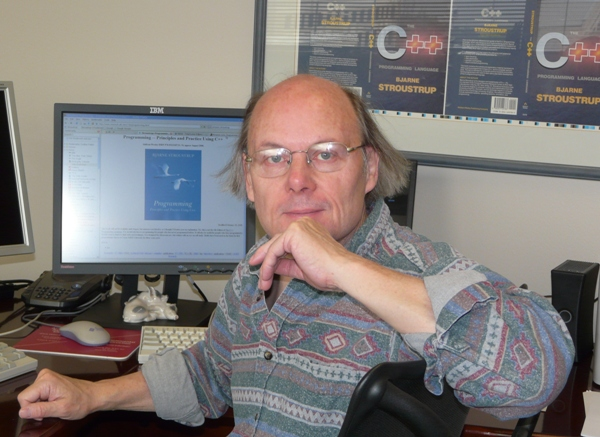
\includegraphics[height=0.25\textheight]{stroustrup}\\
    {\tiny B. Stroustrup, *1950}
  \end{columns}

  \vspace{0.5em}
  \begin{itemize}
  \item C++: C with Objects
  \item A compiler for C++98 exists for virtually all operating
    systems
  \item \dots but not yet for \emph{C++11} (old machines with old OS)
  \item $\Rightarrow$ C++11 is explicitly marked
  \end{itemize}
\end{frame}

\begin{frame}
  \frametitle{Features of C++}
  \begin{description}
  \item[C++ is compatible with C.] \emph{Was} important, now a problem.
  \item[C++ is an imperative, procedural programming language.]
  \item[C++ is an object-oriented programming language.]
  \item[C++ is a compiled language.] The code is translated
    (\textit{compiled}) into machine code by a \textit{compiler}.
  \item[C++ can be used for low-level programming.] Hardware can be
    programmed pretty directly.
  \item[C++ can be used for high-level programming.] Complex
    programs and complex libraries can be implemented.
  \item[C++ is (pretty much) portable.] A C++ compiler exists for
    virtually any platform. However, the dialects vary.
  \item[C++ has libraries for anything.] 
  \item[C++ is used for almost anything.] Many application programs
    are implemented in C++.
  \end{description}
\end{frame}

\begin{frame}
  \frametitle{Level of Abstraction}
  \centering
  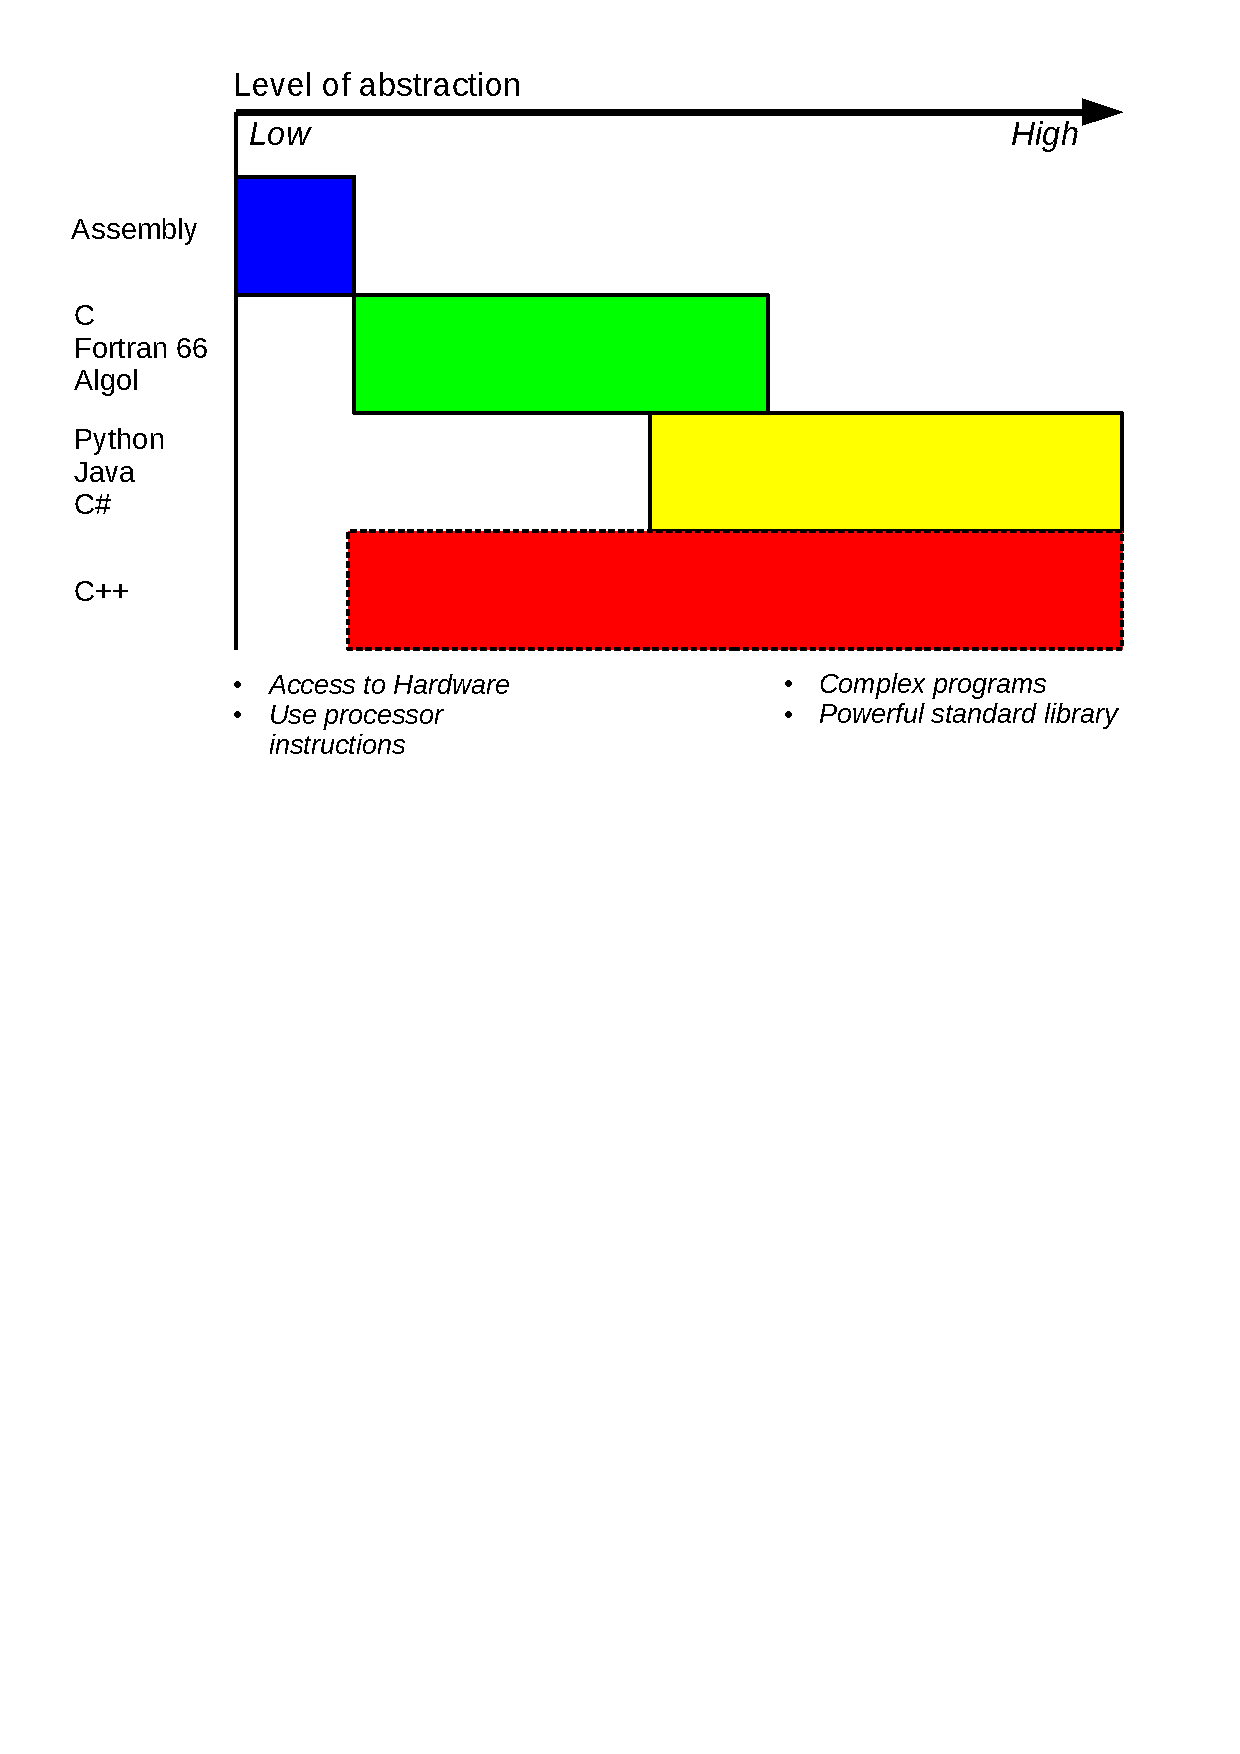
\includegraphics[width=0.9\textwidth]{languages}
\end{frame}

\begin{frame}
  \frametitle{On the Other Hand}
  \centering
  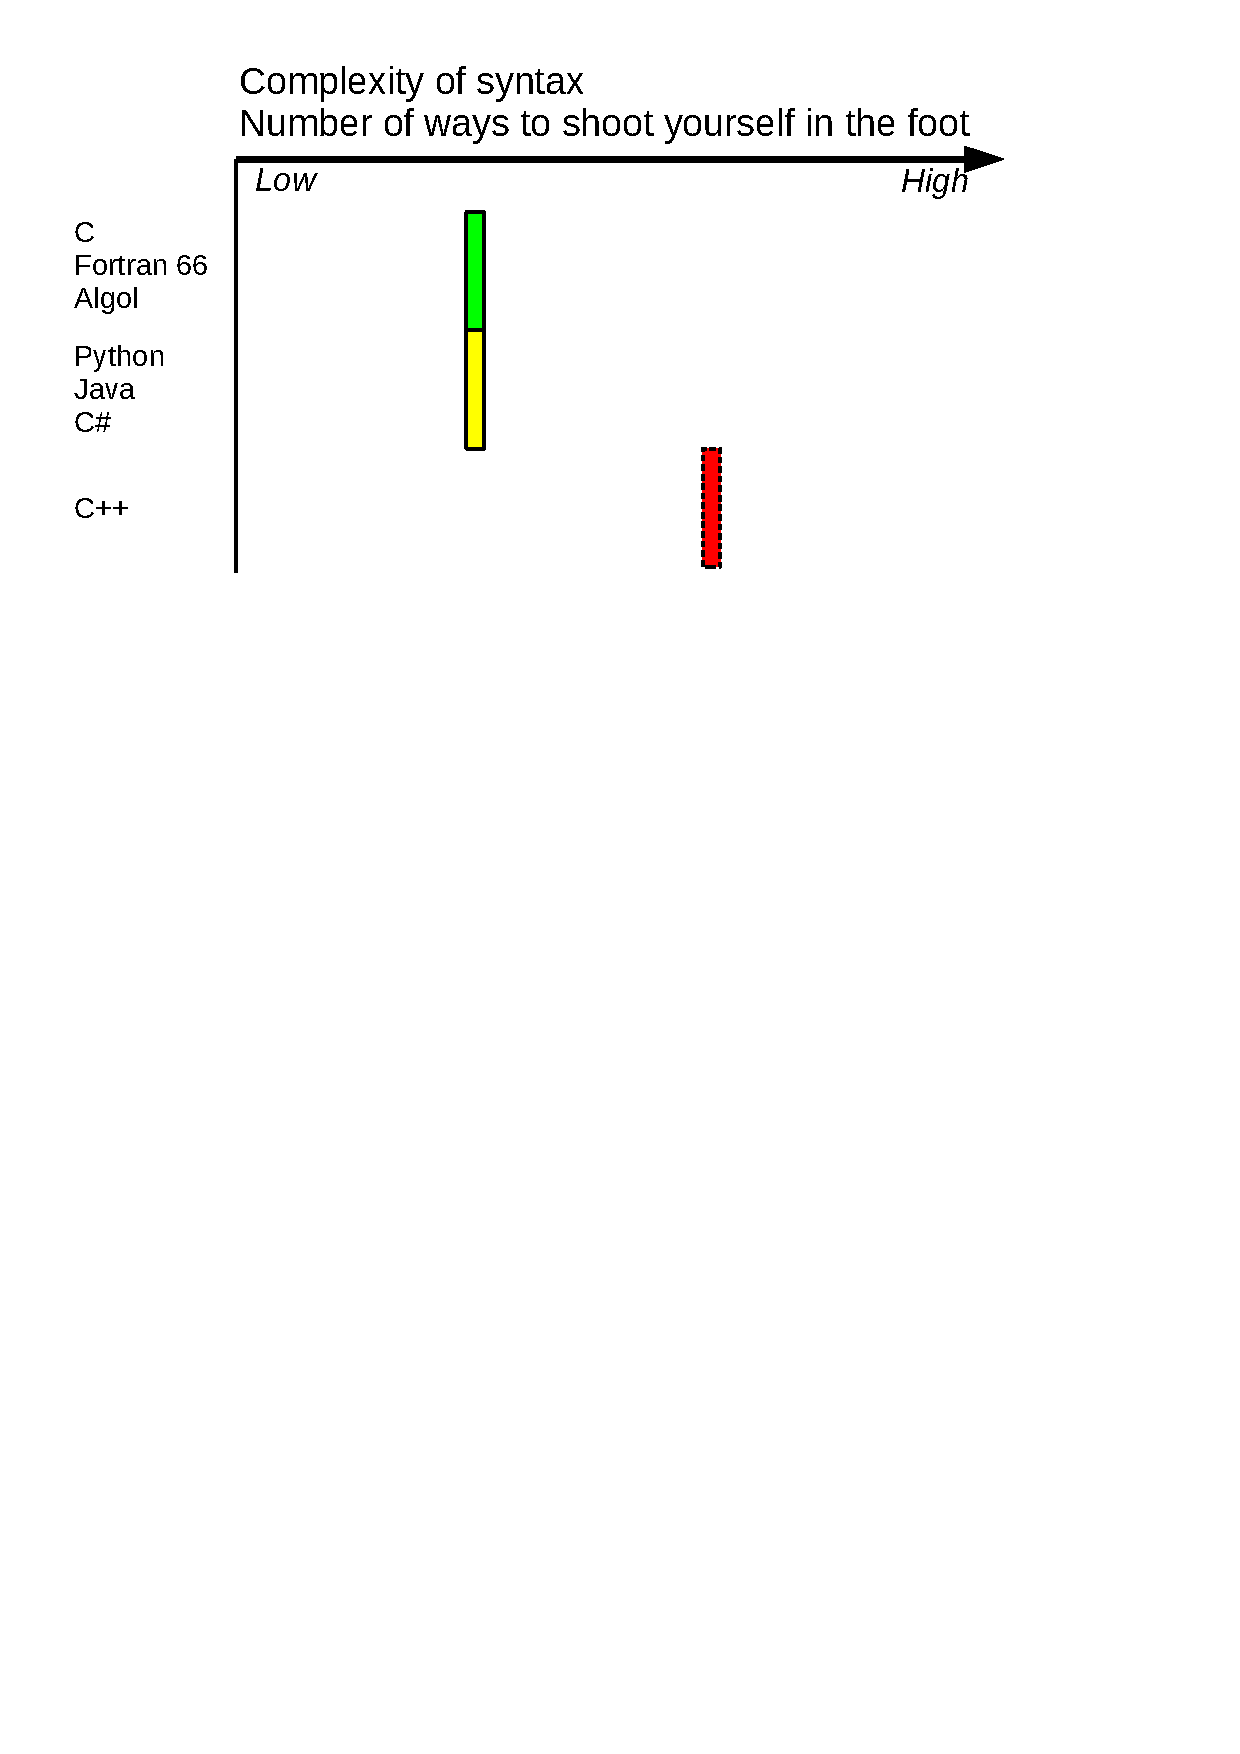
\includegraphics[width=0.9\textwidth]{complexity}
\end{frame}

\begin{frame}
  \vfill
  \centering
  \Huge Let's go \dots
  \vfill
\end{frame}

\end{document}
